\documentclass{beamer}

\usepackage[polish]{babel}
\usepackage[utf8]{inputenc}
\usepackage[T1]{fontenc}
\usepackage{eurosym}

\usetheme{Rochester}

\title[Tablica LED]{Sterownik matrycy świetlnej w~oparciu o~mikrokontroler AVR}
\author{Mikołaj Błajek, Michał Słomkowski, Filip Rachwalak \newline \newline Promotor: dr inż.  Roman Mielcarek}
\institute{Politechnika Poznańska}
\date{7 lutego 2014}

\begin{document}

% TYTUŁ
\begin{frame}
	\titlepage
\end{frame}

% COMMENT
\begin{frame}
	\begin{block}{Cele}
		\begin{itemize}
			\item Zaprojektowanie i~wykonanie sterownika diodowej matrycy świetlnej,
			\item zaimplementowanie programu dla komputera PC umożliwiającego tworzenie animacji tekstowych i~graficznych.
		\end{itemize}
	\end{block}
\end{frame}

% 
\begin{frame}{Schemat blokowy}
	\begin{figure}[h]
		\centering
		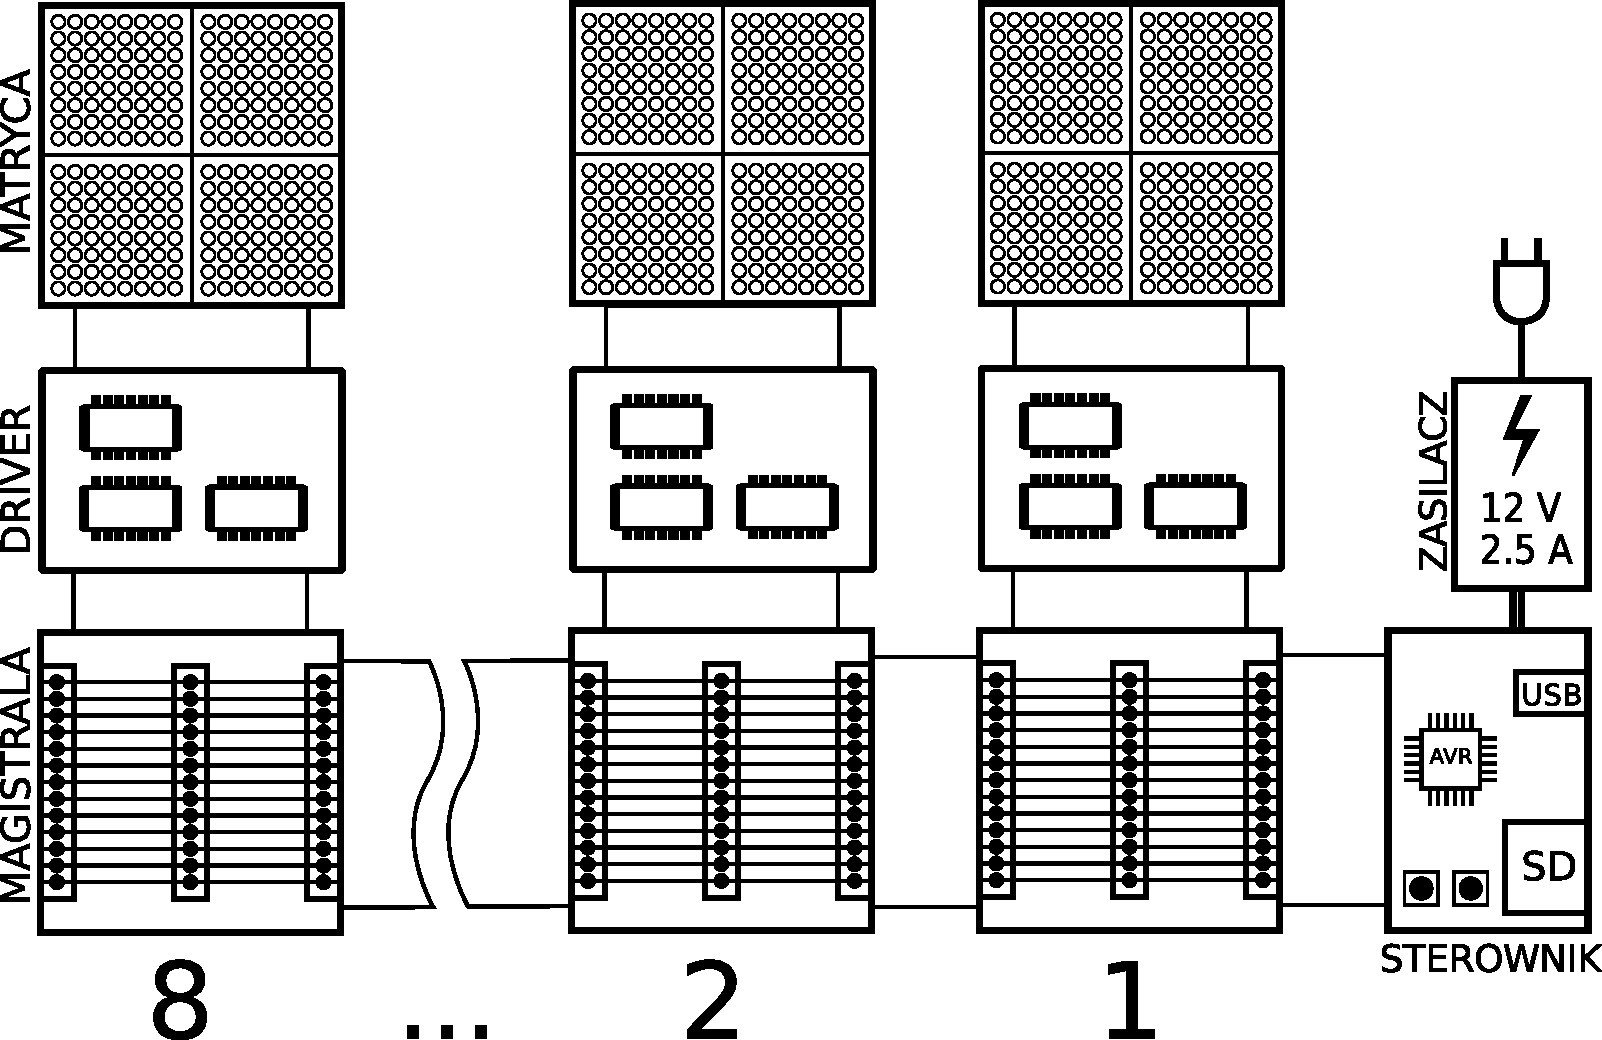
\includegraphics[width=\textwidth]{img/blokowy.pdf}
	\end{figure}
\end{frame}

% 
\begin{frame}{Schemat sterownika}
	\begin{figure}[h]
		\centering
		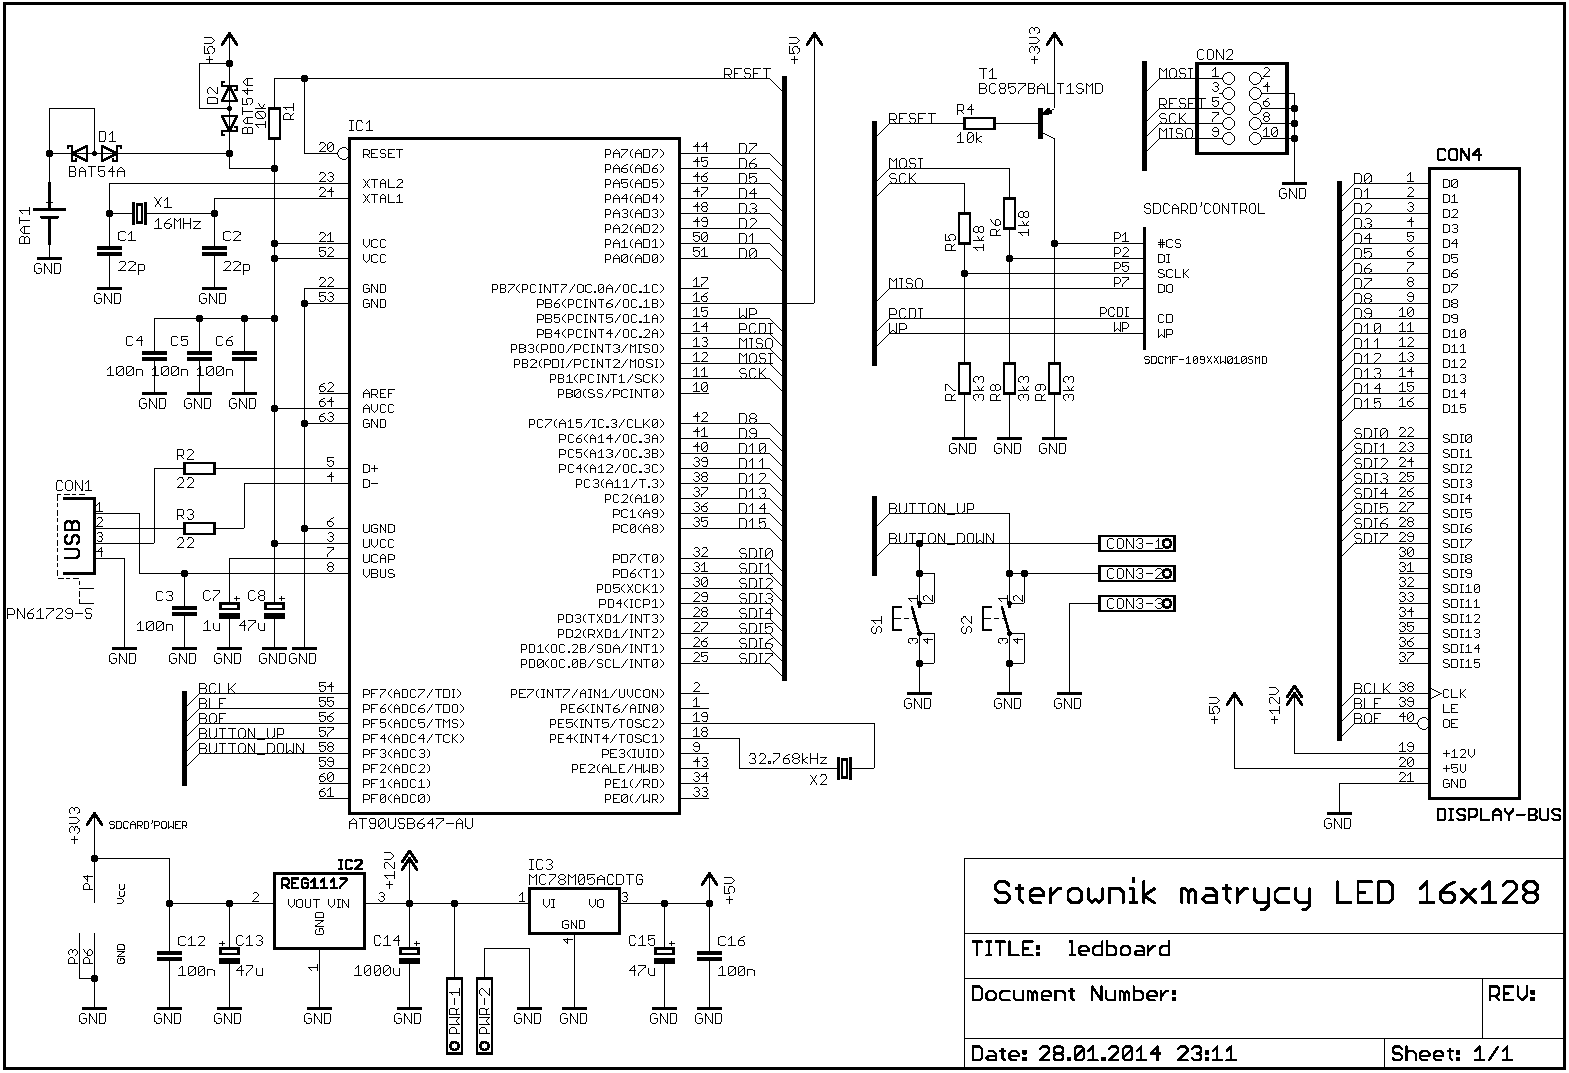
\includegraphics[width=\textwidth]{img/schemat.pdf}
	\end{figure}
\end{frame}

% SCHEMAT STEROWNIKA
\begin{frame}{Wzór ścieżek płytki drukowanej}
	\begin{figure}[h]
		\centering
		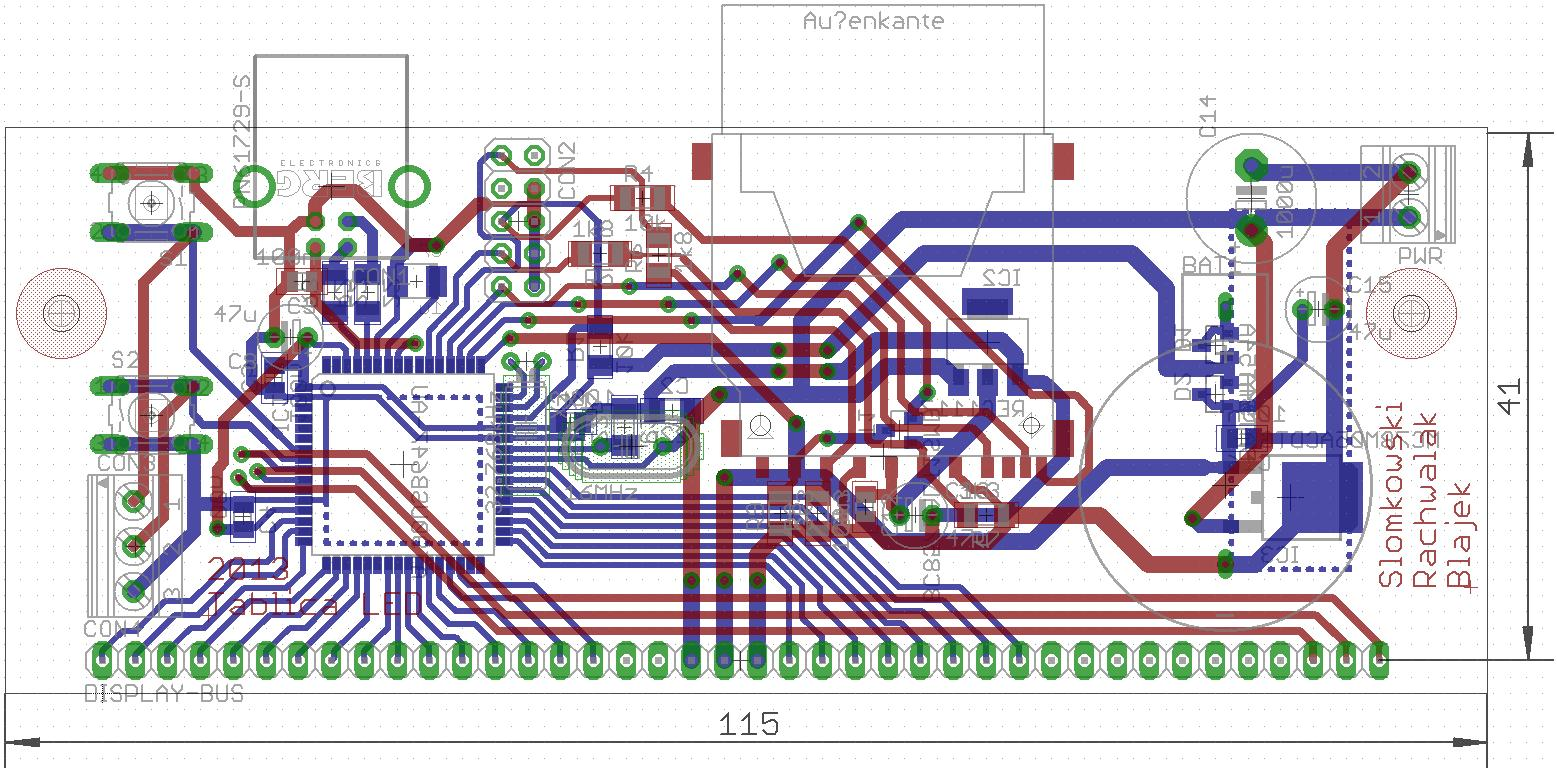
\includegraphics[scale=0.2]{img/schemat.jpg}
	\end{figure}
\end{frame}

% FOTKA PŁYTKI
\begin{frame}{Płytka drukowana sterownika}
	\begin{figure}[h]
		\centering
		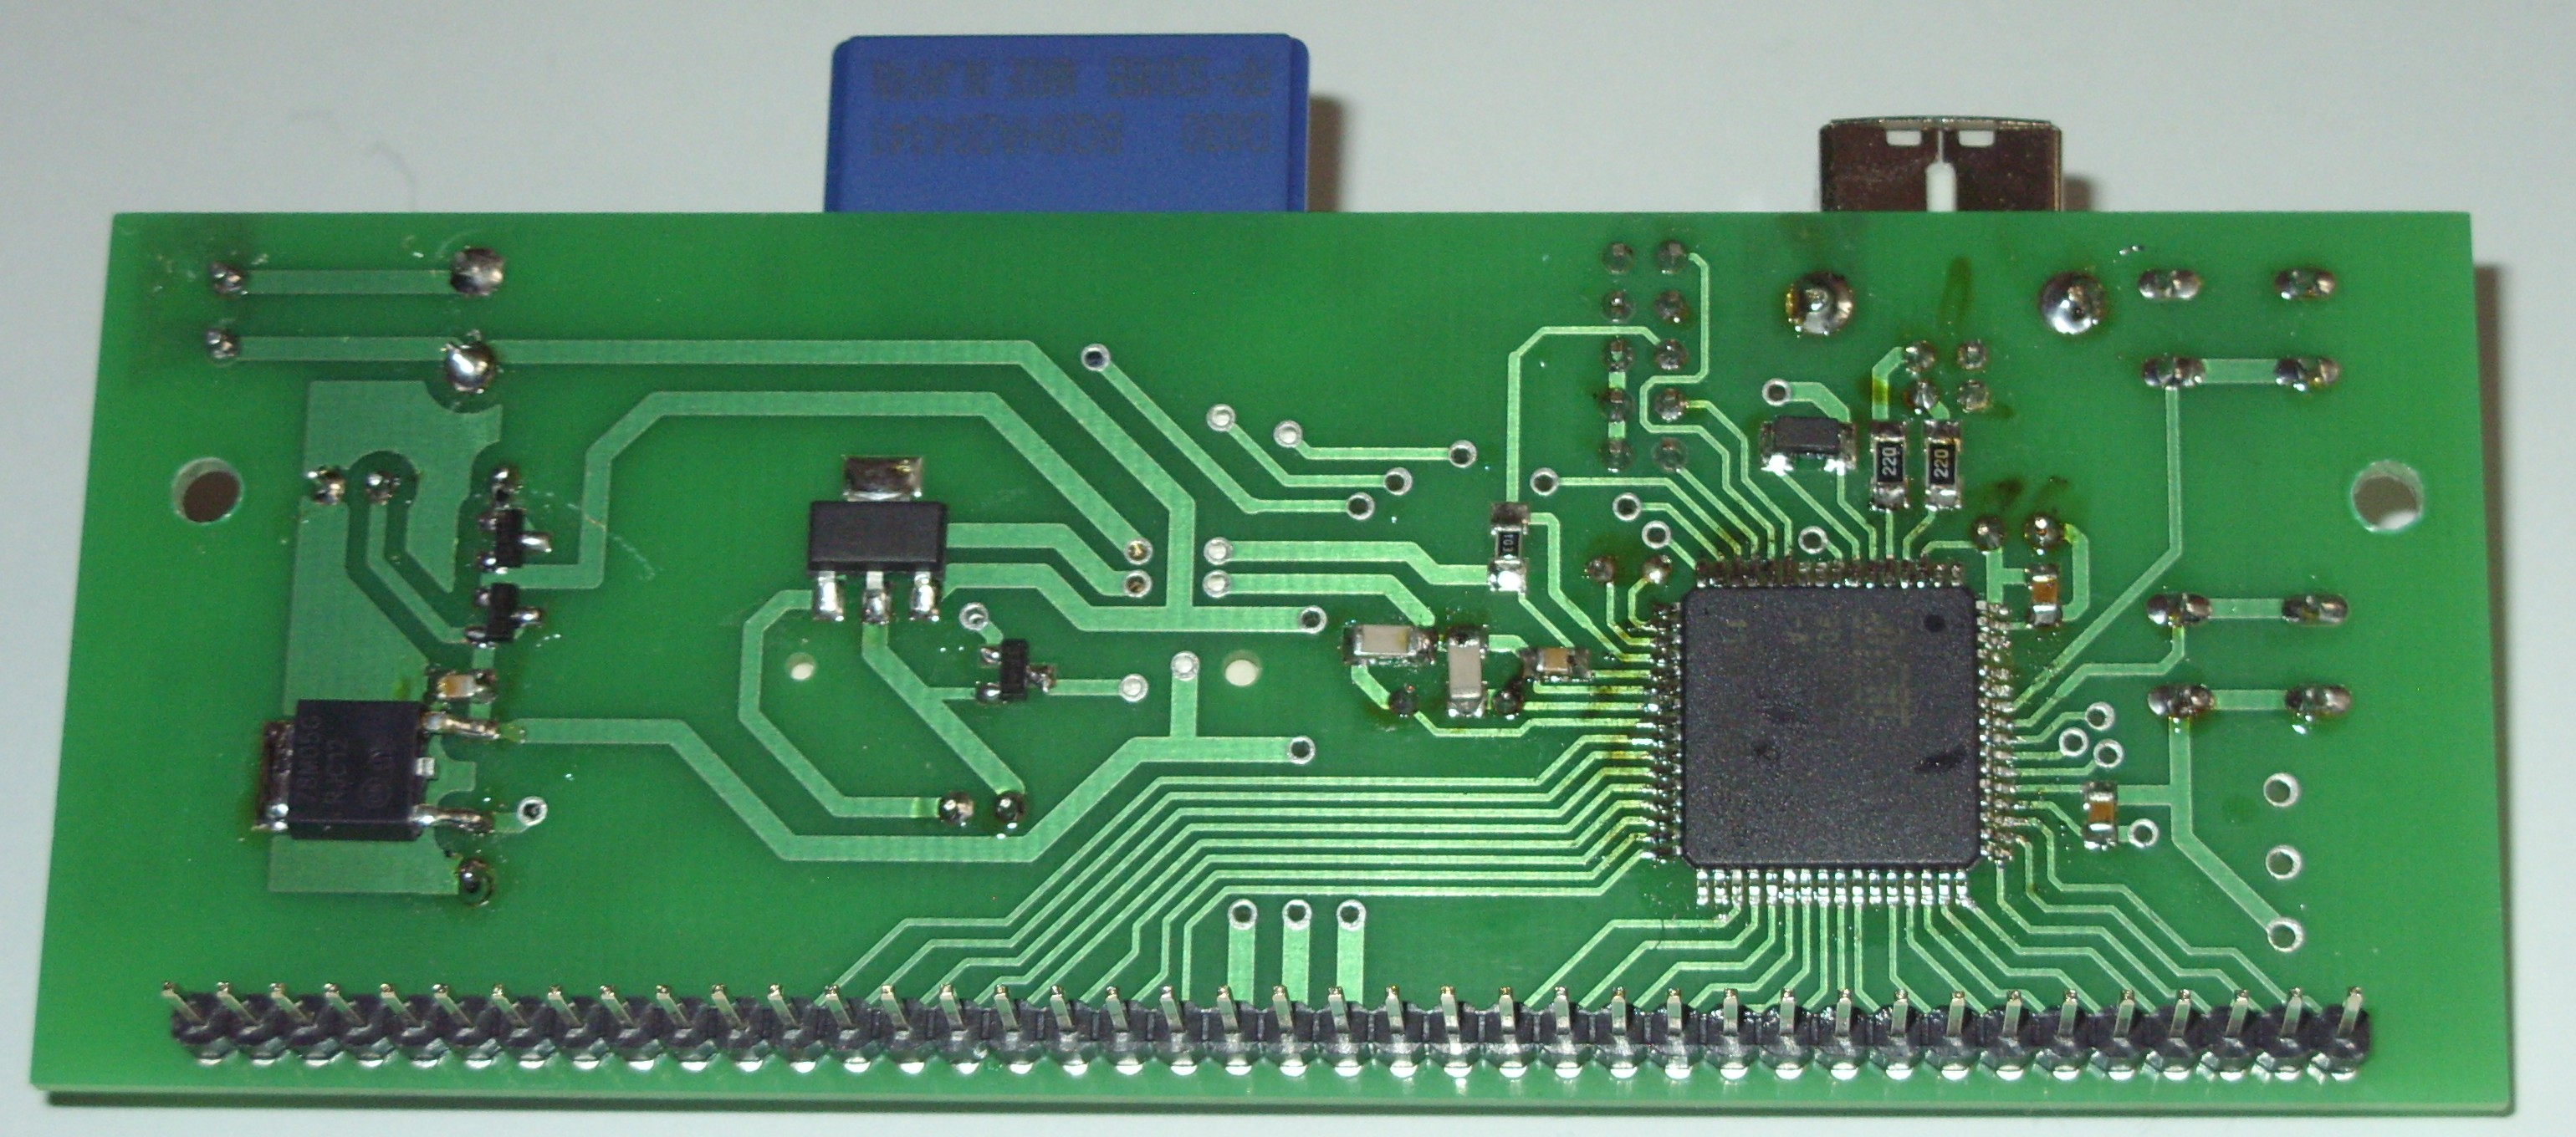
\includegraphics[width=\textwidth]{img/zdj-sterownik-down.jpg}
	\end{figure}
\end{frame}

% FOTKA PŁYTKI
\begin{frame}{Matryca}
	\begin{figure}[h]
		\centering
		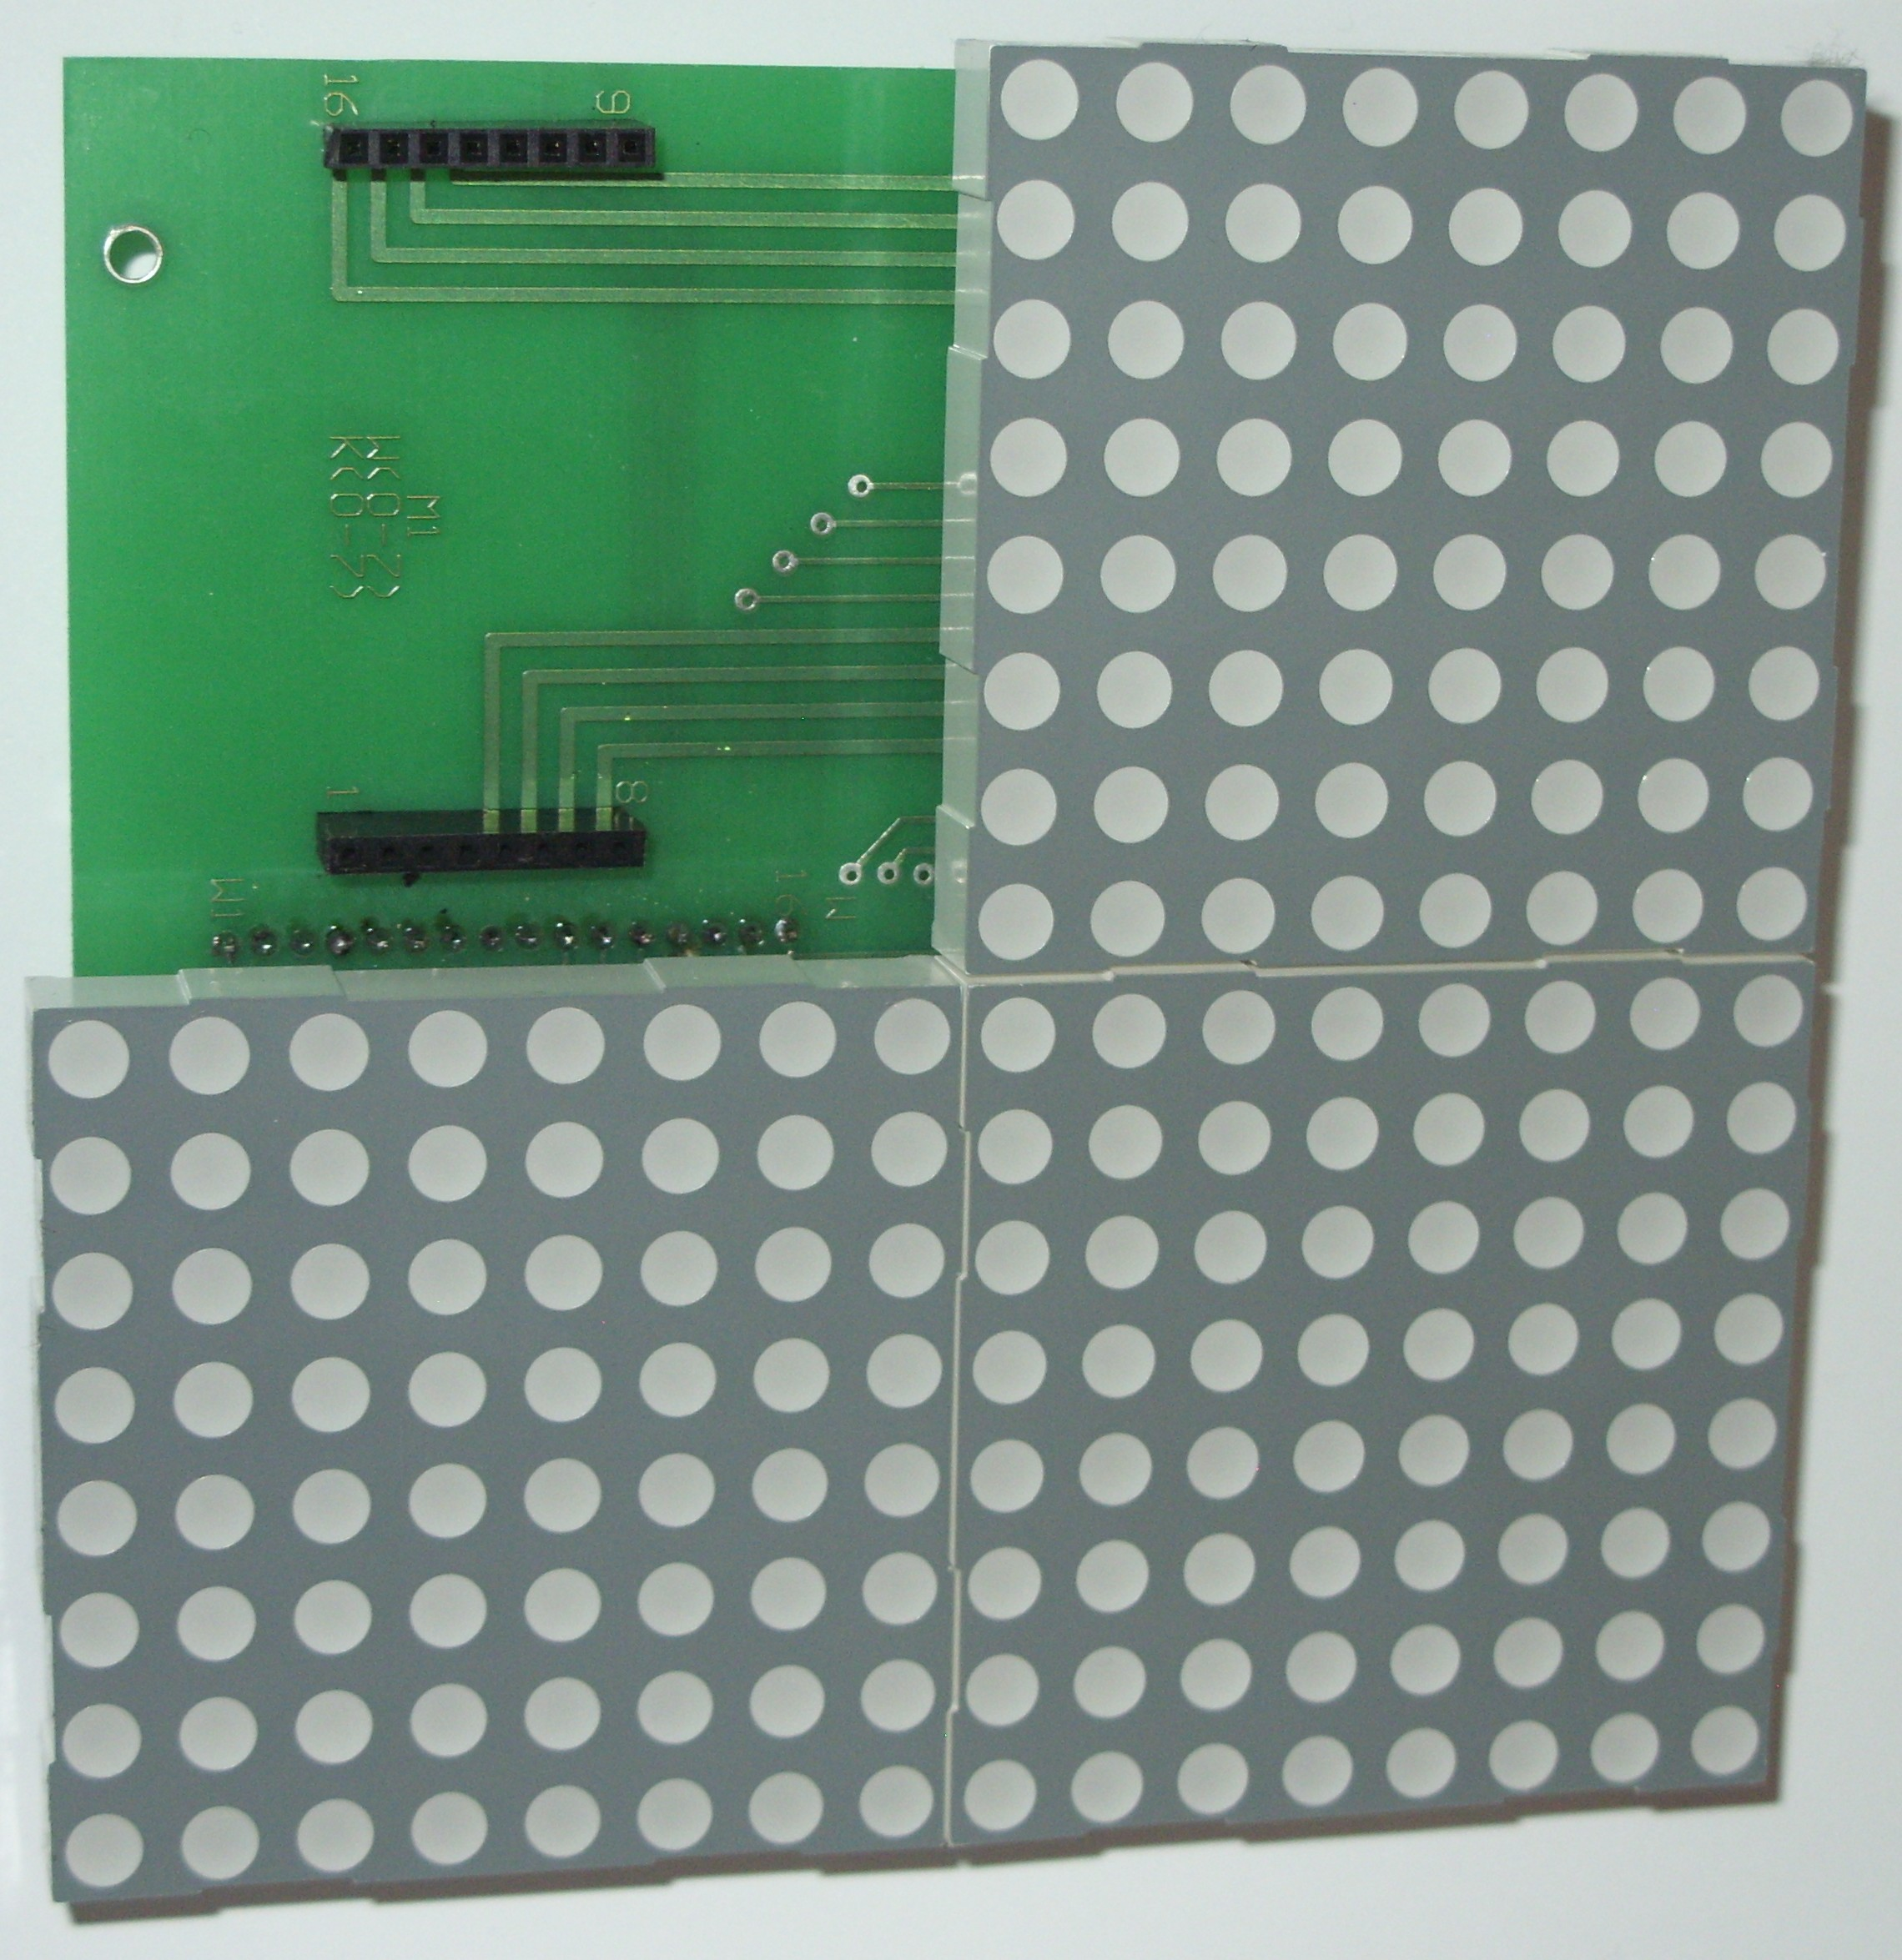
\includegraphics[scale=0.09]{img/matryca.jpg}
	\end{figure}
\end{frame}

% FOTKA PŁYTKI
\begin{frame}{Driver}
	\begin{figure}[h]
		\centering
		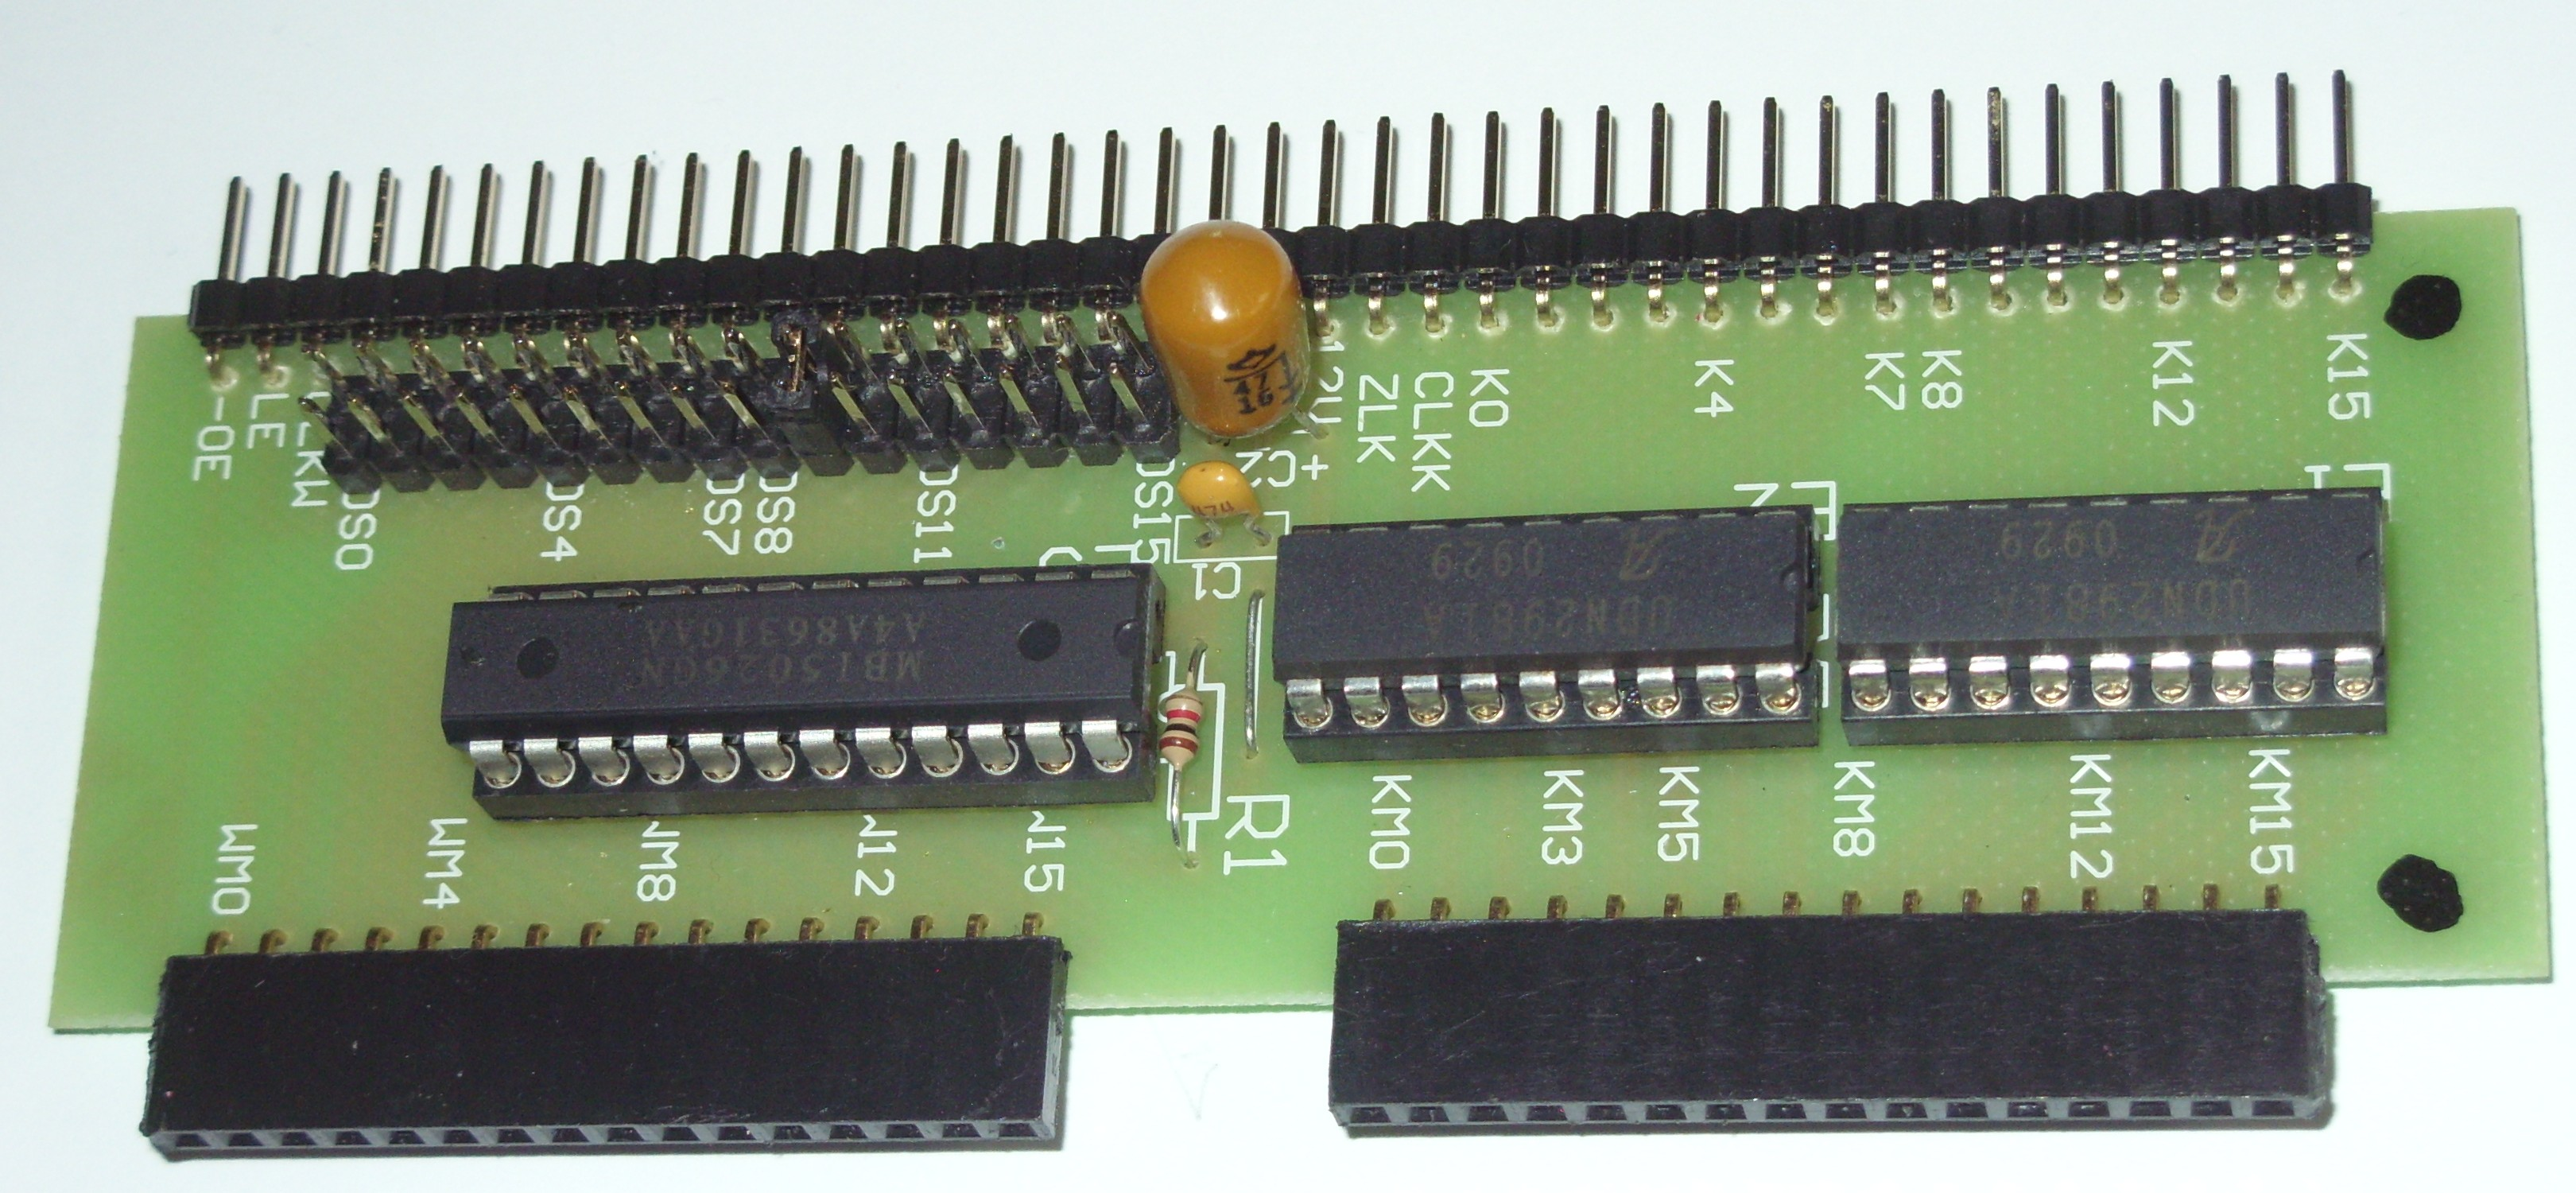
\includegraphics[width=\textwidth]{img/zdj-driver.jpg}
	\end{figure}
\end{frame}

% FOTKA PŁYTKI
\begin{frame}{Firmware --- użyte biblioteki}
	\begin{itemize}
		\item sd\_raw --- biblioteka niskopoziomowej obsługi kart SD,
		\item LUFA --- biblioteka obsługi różnych klas USB dla mikrokontrolerów,
		\item FAT --- biblioteka obsługi systemu plików FAT32.
	\end{itemize}
\end{frame}

% Komendy
\begin{frame}{Plik animacji \texttt{.m2f}}
	\begin{block}{Wymagania}
		\begin{itemize}
			\item wypisywanie aktualnej daty i czasu,
			\item wyświetlanie grafiki i tekstu,
			\item dynamika tekstu (ruch, efekty),
			\item efektywne działanie na mikrokontrolerze.
		\end{itemize}
	\end{block}
\end{frame}

% Komendy
\begin{frame}{Format pliku animacji}
	\begin{block}{Komendy sterujące: \texttt{0,X}}
		\begin{itemize}
			\item koniec,
			\item odczekanie pewnej liczby klatek,
			\item odczekanie do końca sekundy, minuty, godziny, dnia,
			\item włączanie i wyłączanie rysowania tła i znaków,
			\item wczytywanie tła,
			\item czekanie na przycisk,
			\item powrót do początku.
		\end{itemize}
	\end{block}
\end{frame}

% Komendy
\begin{frame}{Format pliku animacji}
	\begin{block}{Komendy modyfikujące litery: \texttt{X, Y, Z}}
		\begin{itemize}
			\item \texttt{X} --- numer znaku w pamięci,
			\item 1--127 (liczba obsługiwanych znaków w sterowniku),
			\item \texttt{Y} --- numer właściwości znaku,
			\item kod znaku, pozycja, przycięcie, tryb wyświetlania, font,
			\item \texttt{Z} --- nowa wartość.
		\end{itemize}
	\end{block}
\end{frame}

% KODOWANIE ZNAKÓW
\begin{frame}{Kodowanie znaków}
	\begin{block}{Znaki}
		\begin{itemize}
			\item 0--11 znaki zastępowane cyframi daty i godziny,
			\item 12, 13: $^\circ$, \euro,
			\item 14--31: Ą--Ż, ą--ż,
			\item 32--126: ASCII,
			\item 127--255: wolne.
		\end{itemize}
	\end{block}
\end{frame}

% CZCIONKI
\begin{frame}{Czcionka 0: 16 pikseli}
	\begin{figure}[h]
		\centering
		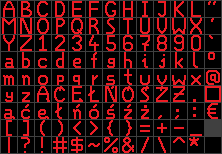
\includegraphics[scale=1.2]{img/czcionka4.png}
	\end{figure}
\end{frame}

% CZCIONKI
\begin{frame}{Czcionka 1: 8 pikseli}
	\begin{figure}[h]
		\centering
		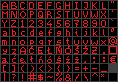
\includegraphics[scale=2.4]{img/czcionkb3.png}
	\end{figure}
\end{frame}

% CZCIONKI
\begin{frame}{Czcionka 2: 12 pikseli}
	\begin{figure}[h]
		\centering
		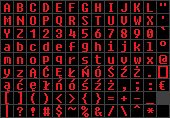
\includegraphics[scale=1.6]{img/czcionkc3.png}
	\end{figure}
\end{frame}

% Program
\begin{frame}{Program do tworzenia animacji}
	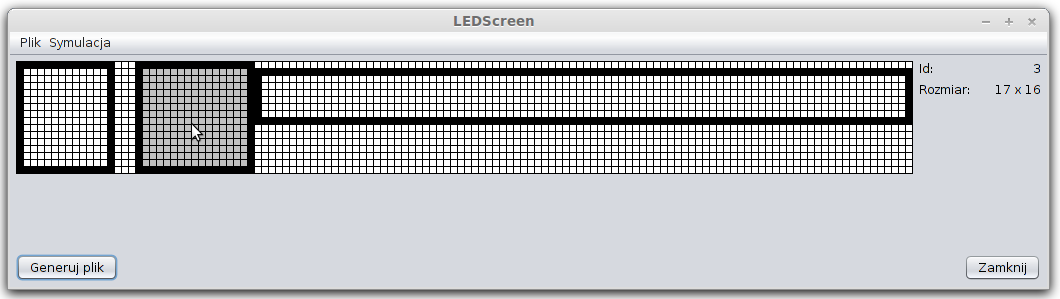
\includegraphics[width=\textwidth]{img/gui2.png}
	\begin{block}{Funkcje programu}
		\begin{itemize}
			\item projektowanie animacji,
			\item zapis projektu w postaci edytowalnej (plik \texttt{.mmf}),
			\item eksport do pliku \texttt{.m2f}.
		\end{itemize}
	\end{block}
\end{frame}

% Program
\begin{frame}{Program do tworzenia animacji}
	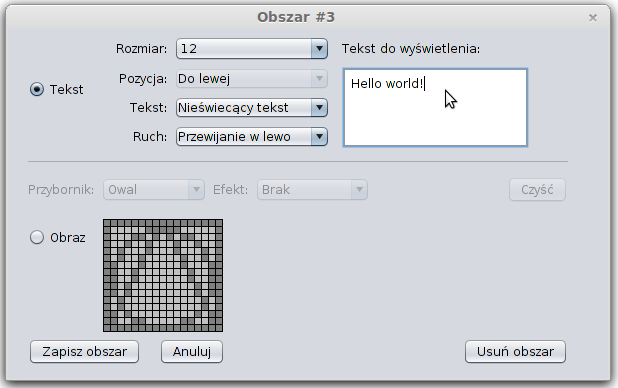
\includegraphics[width=\textwidth]{img/areaText.png}
\end{frame}

\end{document}
